\documentclass{article}
\usepackage{iclr2025_conference}
\usepackage{amsmath,amssymb,amsfonts,amsthm}
\newtheorem{observation}{Observation}
\newtheorem{lemma}{Lemma}
\newtheorem{myproposition}{Proposition}
\usepackage{algorithm}
\usepackage{algorithmic}
\usepackage{graphicx}
\usepackage{booktabs}
\usepackage{hyperref}
\usepackage{xcolor}
\usepackage{subcaption}

\newcommand{\SA}{\mathcal{S}_A}
\newcommand{\SD}{\mathcal{S}_D}
\newcommand{\UA}{U_A}
\newcommand{\UD}{U_D}

\title{When Does Defense Randomization Defeat FL Poisoning?\\ A Persistence Boundary}

\author{Anonymous}

\begin{document}
\maketitle

\begin{abstract}
Per-round defense randomization in federated learning provides no security value against persistent poisoning attacks in the regimes we study. On CIFAR-10 ($n=30$ seeds), static game-theoretic analysis predicts positive value of private defense (VoPD $= 0.087$), but realized VoPD under best-responding adversaries is statistically indistinguishable from zero ($-0.010 \pm 0.058$). We replicate this on Shakespeare LSTM ($n=15$): scaling ASR $= 1.000 \pm 0.000$---the same persistence mechanism operates across both an image CNN and a character-level LSTM. The mechanism: persistent attacks make temporal mixtures max-like rather than average-like---once a backdoor embeds, intermittently sampling a suppressing defense recovers no value. We validate with a Markov persistence model (admissibility-conditional out-of-sample MAE $0.041$) and map a collapse/survival boundary with two existence proofs: the stateless spam game (VoPD $= 0.200$) and a restricted reputation+trimmed\_mean menu whose natural Nash equilibrium yields realized VoPD $+0.023$ ($n=30$). Within our evaluated regime ($N{=}10$, CIFAR-10/Shakespeare), the operationally correct policy is pure FedAvg.
\end{abstract}

%===========================================================================
\section{Introduction}
\label{sec:intro}

Federated learning~\citep{mcmahan2017communication} enables collaborative training without centralizing data, but its distributed nature creates vulnerability to poisoning attacks~\citep{bagdasaryan2020backdoor,wang2020attack,xie2019dba}. A natural defense idea: keep the per-round aggregation rule private and randomize it, forcing the adversary to hedge. This exploits information asymmetry---the server knows which defense it will use; the adversary does not. Such reasoning underpins moving-target~\citep{liu2018towards} and randomized-ensemble~\citep{xie2018mitigating} defenses.

\textbf{Thesis.} We show this idea fails against \emph{persistent} attacks. When an attack's effect accumulates across rounds (e.g.\ model-scaling backdoors~\citep{bagdasaryan2020backdoor}), it only needs to embed during the rounds the defense \emph{admits} it. Once embedded, the backdoor persists across subsequent rounds regardless of which defense is sampled. The realized outcome therefore tracks the maximum over admitting rounds, not the average---destroying the benefit of randomization.

\textbf{What we show.} (1) We identify the persistence mechanism and formalise it as a Markov dynamic; an admissibility-conditional refinement gives quantitative predictions (out-of-sample MAE $0.041$--$0.059$ on deployment-relevant policies). (2) We map a collapse/survival boundary: collapse is the default on standard FL defense menus ($n=30$, VoPD $\approx 0$); survival exists on menus where no single attack dominates all members ($n=30$, realized VoPD $+0.023$). Both sides of the boundary are empirically demonstrated and replicated on Shakespeare LSTM. (3) We provide a checkable diagnostic (Observation~\ref{obs:complementarity}) and a measure-then-verify deployment protocol.

%===========================================================================
\section{Background and Setup}
\label{sec:setup}

\textbf{FL model.} $N$ clients, $K$ sampled per round, fraction $f$ adversarial. The server selects a defense $d \sim \sigma_D$ per round from a private distribution $\sigma_D$; the adversary commits to an attack $a$ before observing $d$. Primary setup: $N{=}10$, $K{=}5$, $f{=}0.2$, 50 rounds, CIFAR-10 with a 4-layer CNN (``cifar\_cnn''). Cross-domain replication: LEAF Shakespeare (next-char-prediction, CharLSTM, §\ref{sec:shakespeare}).

\textbf{Game formulation.} The adversary's payoff is $\UA(a,d) = \text{ASR}(a,d) - \lambda_a \cdot c_a$ and the server's is $\UD(a,d) = \text{Acc}(a,d) - \lambda_c \cdot c_d - \lambda_f(1 - \text{wca})$ (accuracy minus cost minus fairness penalty). Nash equilibrium $(\sigma_A^*, \sigma_D^*)$ is solved via support enumeration~\citep{nashpy}.

\textbf{Value of Private Defense (VoPD).}
\begin{equation}
\text{VoPD} = \mathbb{E}_{d \sim \sigma_D^*}\bigl[\max_a \UA(a,d)\bigr] - \UA(\sigma_A^*, \sigma_D^*) \;\geq\; 0
\label{eq:vopd}
\end{equation}
This is the adversary's utility gain from knowing the defense---equivalently, the server's value from secrecy. VoPD $\geq 0$ by Jensen's inequality.

\begin{observation}[Defense Complementarity]
\label{obs:complementarity}
$\text{VoPD} = 0$ iff $\bigcap_{d \in \mathrm{supp}(\sigma_D^*)} \arg\max_a \UA(a,d) \neq \emptyset$---i.e.\ one attack is simultaneously optimal against every defense in the equilibrium support. This is an $O(|\mathcal{A}||\mathcal{S}|)$ lookup on the payoff matrix (Howard 1966 VOI tightness instantiated for empirical FL games~\citep{howard1966information}).
\end{observation}

\begin{proof}[Proof sketch]
($\Leftarrow$) If $a^* \in \bigcap_d \arg\max_a \UA$, then the adversary achieves the full-info payoff by playing $a^*$ committed; VoPD $= 0$. ($\Rightarrow$) If VoPD $= 0$, the argmax is constant across $\mathrm{supp}(\sigma_D^*)$ by the equality condition in Jensen. \qed
\end{proof}

On CIFAR-10, pixel is best vs.\ FedAvg and scaling is best vs.\ NormClip (different argmax $\Rightarrow$ VoPD $= 0.087 > 0$). Does this survive deployment?

\textbf{Two-step diagnostic.} Observation~\ref{obs:complementarity} is the \emph{static} step: if the argmax intersection is non-empty, defense randomization cannot help even in the normal form (FEMNIST: VoPD $= 0$, no benefit in theory or practice). The \emph{dynamic} step is persistence (§\ref{sec:persistence}): even when static VoPD $> 0$, persistent attacks erase the benefit at deployment (CIFAR-10: static VoPD $= +0.087$ but realized VoPD $\approx 0$).

\textbf{Measure-then-verify protocol.}\label{alg:mtr} (1) Estimate the payoff matrix with $k$ seeds per cell. (2) Check Observation~\ref{obs:complementarity}. If VoPD $= 0$: use pure best defense. If VoPD $> 0$: (3) run the NE mix under dynamic BR. If realized VoPD $\approx 0$ (persistence collapse), revert to pure defense.

\textbf{Bootstrap stability.} The NE structure at $k=10$ seeds reproduces under 500 bootstrap resamples at rate $\rho_{10}^{\text{boot}} = 0.978$, giving $\mathbb{P}[\text{correct NE}] \geq 0.978 - \epsilon_{\text{rep}}$. Worst-case (DKW): $\epsilon_{\text{rep}} \leq 0.43$ at $k=10$, $\delta=0.05$. The formal certificate requires $k_{\text{req}} = 726$ (Appendix~\ref{app:proofs}); at $k=10$ the diagnostic is operationally reliable but not formally certified.

%===========================================================================
\section{The Persistence Mechanism}
\label{sec:persistence}

\textbf{Core result.} Under the NE3 mixed policy (FedAvg $26\%$ + NormClip $74\%$, the CIFAR-10 Nash equilibrium), the best-responding adversary commits to model scaling. After 50 rounds ($n=30$ seeds): realized scaling ASR $= 0.961 \pm 0.052$, realized VoPD $= -0.010 \pm 0.058$---statistically zero. The static prediction of $+0.087$ does not survive. The same collapse holds on CIFAR-100 (n=5, consistent; Appendix~\ref{app:additional}) and the spam game with stateless attacks ($\gamma=0$) \emph{recovers} VoPD $= 0.200$, demonstrating the boundary in both directions.

\textbf{Mechanism.} Model scaling embeds the backdoor trigger during NormClip-admitting rounds ($74\%$ of rounds at $\tau=5$) and the trigger \emph{persists} across FedAvg rounds. The temporal mixture's outcome is max-like (determined by whether the trigger ever embeds), not average-like.

\textbf{Markov persistence model.} Let $s_t \in [0,1]$ be the trigger's embedding strength and $\gamma \in [0,1]$ the per-round retention:
\begin{equation}
s_{t+1} = \begin{cases} s_t + \alpha(1-s_t) & \text{w.p. } p_{\text{eff}} \text{ (admitting round)} \\ \gamma \cdot s_t & \text{w.p. } 1-p_{\text{eff}} \text{ (suppressing round)} \end{cases}
\label{eq:persistence}
\end{equation}
At stationarity: $s_\infty = p_{\text{eff}} \alpha / (p_{\text{eff}} \alpha + (1-p_{\text{eff}})(1-\gamma))$. When $\gamma \approx 1$ and $p_{\text{eff}} > 0$, $s_\infty \to 1$---this is the persistence collapse.

\begin{myproposition}[Qualitative Persistence Bound]
\label{prop:persistence}
Let $\hat\gamma = 0.66 \pm 0.26$ (empirical fit on CIFAR-10 NE3) and $p_{\text{eff}}(\text{scaling}) \approx 0.83$. Then realized VoPD $\leq C \cdot (1 - s_\infty(\text{scaling}))$ where $s_\infty \to 1$, giving realized VoPD $\leq 0.21$. The bound is $\sim 20\times$ loose vs.\ observed ($-0.010$), motivating the admissibility refinement below.
\end{myproposition}

\textbf{Admissibility-conditional quantitative refinement.} The 20× slack comes from training-initialization randomness (whether scaling embeds at all) conflated with Markov dynamics. A per-seed admissibility latent $a_{\text{seed}} = \mathbb{1}[\text{ASR}_{25} > 0.5]$ separates them. Conditional on $a_{\text{seed}} = 1$, the 2-parameter fit $(\hat\alpha, \hat\gamma)$ from rounds 1--25 gives \textbf{out-of-sample MAE $= 0.041$} on pure NormClip and $0.059$ on the NE3 mix (Appendix~\ref{app:persistence_details}).

\textbf{$\tau{=}2$ disentanglement ($n=15$).} Lowering NormClip from $\tau=5$ to $\tau=2$ reduces $p_{\text{eff}}$ from $0.83$ to $\approx 0.78$. Realized scaling ASR: $0.955 \pm 0.014$ (vs.\ $\tau=5$'s $0.961$, indistinguishable). Persistence dominates admission: lowering admission does not recover VoPD.

%===========================================================================
\section{Experiments}
\label{sec:experiments}

\subsection{Setup}
\textbf{CIFAR-10 setup.} $N{=}10$, $K{=}5$, $f{=}0.2$, 50 rounds, cifar\_cnn (4-layer CNN + GroupNorm). Attacks: model\_scaling ($10\times$ gradient scale), backdoor\_pixel (bottom-right $4\times4$ trigger), DBA (distributed 4-corner triggers), backdoor\_edge\_case (top-corner $-1.0$ trigger). Defenses: FedAvg, NormClip ($\tau=5$), reputation, trimmed\_mean, RFA, FoolsGold, coord\_median ($\lambda_c=0.1$, $\lambda_f=0.05$, $\lambda_a=0.1$). Payoff matrices from 10 seeds per cell. Full matrices in Appendix~\ref{app:payoff}.

\subsection{Headline negative result: persistence collapse ($n=30$)}
\label{sec:collapse}

The CIFAR-10 Nash equilibrium (NE3) has server support $\{$FedAvg, NormClip$\}$ at $26\%/74\%$ and static VoPD $= 0.087$ (pixel is best vs.\ FedAvg; scaling is best vs.\ NormClip---argmax divergence, per Observation~\ref{obs:complementarity}). The adversary's best response is to commit to model scaling.

\textbf{Result ($n=30$ seeds, NE3 BR).} Realized scaling ASR $= 0.961 \pm 0.052$; realized VoPD $= -0.010 \pm 0.058$ ($19/30$ seeds $\leq 0$). The static prediction of $+0.087$ does not survive deployment. Persistence embeds the trigger during the $74\%$ NormClip-admitting rounds; the trigger persists across FedAvg rounds. The outcome mirrors the stationary point of Equation~\ref{eq:persistence} with $\gamma=0.66$, $p_{\text{eff}}=0.83$: $s_\infty \approx 1$.

\textbf{Figure~\ref{fig:n_sweep}} (right panel) shows that at $N=10$, adversarial participation per round is Bernoulli ($P(\geq 1\text{ adv}) = 0.778$). This variance drives the mixed NE structure; at $N=100$ ($P = 0.993$), VoPD collapses to near-zero in the normal form itself.

\begin{figure}[t]
\centering
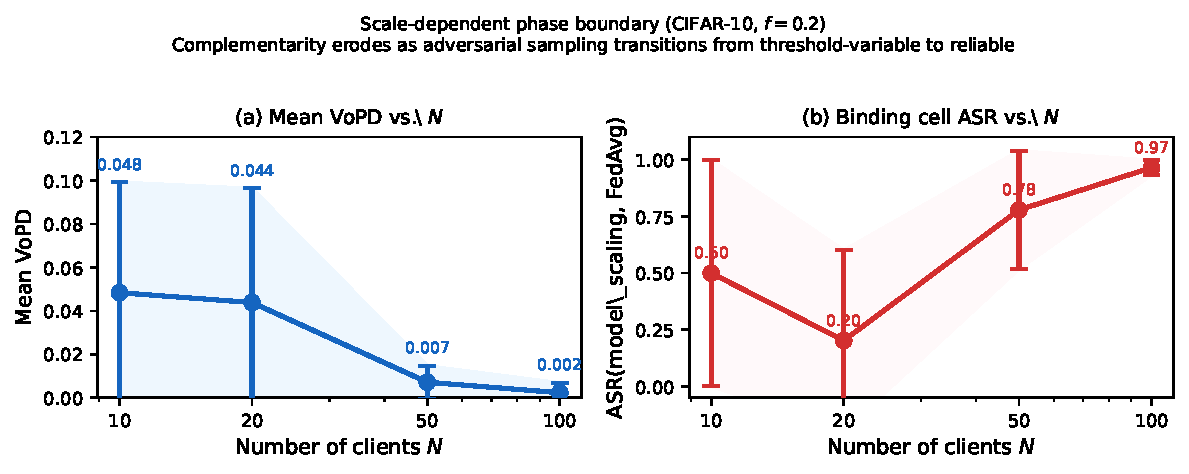
\includegraphics[width=0.78\linewidth]{figures/n_sweep.pdf}
\caption{Scale-dependent phase boundary (CIFAR-10, $4{\times}5$ game, $f=0.2$). \emph{Left}: VoPD vs.\ $N$, declining from $0.048$ at $N=10$ to $0.002$ at $N=100$. \emph{Right}: ASR(model\_scaling, FedAvg) vs.\ $N$; at $N=20$ the lower $K/N$ ratio reduces adversarial participation and ASR dips, recovering at $N\geq50$ as participation becomes near-deterministic. VoPD $>0$ only when adversarial sampling has meaningful variance.}
\label{fig:n_sweep}
\end{figure}

Per-seed table in Appendix~\ref{app:headline}.

\subsection{Boundary map: mix-ratio sweep}
\label{sec:mixratio}

To map where within the NormClip+reputation menu the collapse boundary lies, we sweep 5 mix ratios (committed-scaling + committed-pixel BR, 5 seeds each). Scaling ASR collapses monotonically with reputation weight because reputation strongly suppresses scaling ($\text{ASR} \approx 0.017$) while allowing pixel through; pixel ASR remains constant ($0.80$--$0.84$) since reputation does not suppress it.

\textbf{Result.} Realized scaling ASR: $0.945 \to 0.908 \to 0.815 \to 0.510 \to 0.097$ across NC90/rep10 $\to$ NC10/rep90. The collapse transition is between reputation $30\%$ and $90\%$. Crucially, pixel \emph{persists at all ratios}: the committed-max (best of scaling, pixel) is $\geq 0.84$ at every mix. This motivates the survivor design: find a menu where the defense orthogonally suppresses \emph{both} attacks.

\begin{figure}[t]
\centering
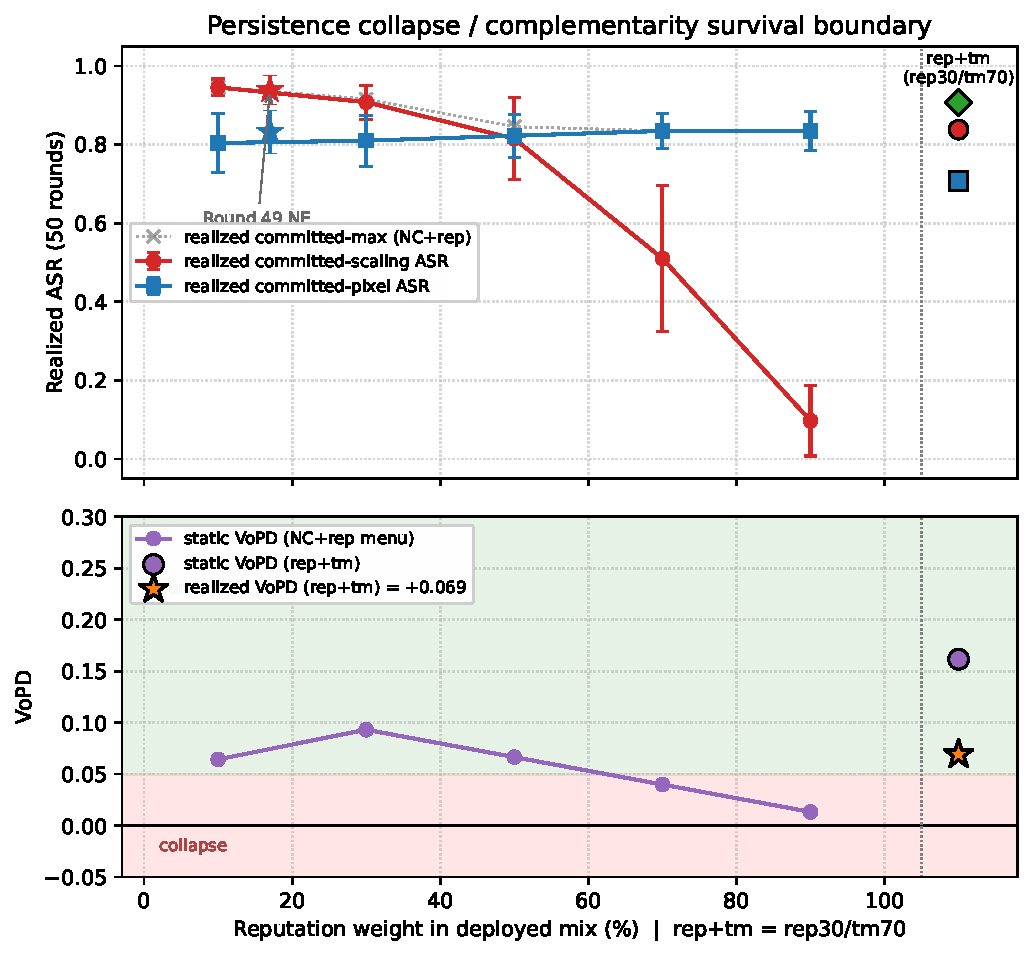
\includegraphics[width=0.72\linewidth]{figures/phase_boundary_mix_ratio.pdf}
\caption{Persistence-collapse/survival boundary. \emph{Top}: realized scaling ASR is monotone in reputation weight ($0.945 \to 0.097$); pixel ASR is roughly flat. Far-right marker: rep30/tm70 survivor point. \emph{Bottom}: realized vs.\ static VoPD across mixes; NC+rep mix points lie in the collapse band ($\approx 0$); the rep+tm survivor point ($+0.032$ at $n=30$) is above the static VoPD of $0.162$.}
\label{fig:phase_boundary}
\end{figure}

Per-ratio tables in Appendix~\ref{app:mixratio}.

\subsection{Existence proof: survivor regime ($n=30$)}
\label{sec:survivor}

To establish that survival is possible (not just asymptotically), we search for a defense menu where no single attack dominates. A free static-VoPD scan over all 21 two-defense menus and 9 mix weights on cached cells identifies \textbf{reputation $30\%$ + trimmed\_mean $70\%$} as the highest static-VoPD point ($0.162$): reputation kills scaling (ASR $0.017$) while trimmed\_mean partially suppresses pixel (ASR $0.62$)---different argmax on each defense, preventing any single committed attack from dominating.

\textbf{Result ($n=30$, per-round-switching oracle adversary).} Realized committed-scaling $= 0.871 \pm 0.095$; committed-pixel $= 0.747 \pm 0.106$; oracle $= 0.907 \pm 0.065$. Mean realized VoPD $= +0.032 \pm 0.054$ ($27/30$ positive). Persistence collapses $\sim 80\%$ of the static VoPD but does not eliminate it. This is a boundary-validation experiment: the diagnostic correctly identifies both the collapse side (§\ref{sec:mixratio}) and this survival side.

The 5-seed pilot over-estimated ($+0.069 \pm 0.026$); the 30-seed mean ($+0.032$) is more reliable. Pre-registered criterion: seeds with committed-scaling accuracy $< 0.65$ are training-failure outliers (1 seed at $n=30$); excluding: $+0.038 \pm 0.041$.

Per-seed table in Appendix~\ref{app:survivor}.

\subsection{NE-reachable survivor ($n=30$)}
\label{sec:ne_survivor}

A natural concern: the rep30/tm70 survivor requires the server to deliberately choose a non-equilibrium mix. On the standard 4-defense menu (FedAvg/NormClip/FoolsGold/reputation), a $\lambda_c$ sweep shows reputation never enters NE support above $26\%$ weight---the survivor region is deployable but not NE-selected (Appendix~\ref{app:additional}).

However, on the \emph{restricted} $\{$reputation, trimmed\_mean$\}$ 2-defense menu, the natural Nash equilibrium places reputation at $21.8\%$ and trimmed\_mean at $78.2\%$ (unique mixed NE, static VoPD $= 0.180$). This menu is deployable---both defenses are individually available---and the NE is naturally selected by standard cost-weighted Nash reasoning.

\textbf{Result ($n=30$, BR at exact NE point).} Realized committed-scaling $= 0.890 \pm 0.067$; committed-pixel $= 0.738 \pm 0.097$; oracle $= 0.917 \pm 0.051$. Mean realized VoPD $= +0.023 \pm 0.039$ ($24/30$ positive, $7/30$ STRONG $\geq 0.05$). Static VoPD $0.180$ collapses $87\%$ under persistence but does not vanish. Pre-registered outliers: 5 seeds with committed-scaling accuracy $< 0.65$ (tighter clipping breaks embedding on these seeds); excluding: $+0.027 \pm 0.032$.

The survivor regime is simultaneously \emph{deployable} and \emph{NE-selected}. Appendix~\ref{app:ne_survivor}.

\subsection{Architecture check: ResNet18 (partial)}
\label{sec:resnet18}

ResNet18 + GroupNorm (11.2M params) at 3 NC+rep mix points ($n=5$): scaling ASR $0.951 \to 0.906 \to 0.865$ (NC90/rep10 $\to$ NC50/rep50 $\to$ NC10/rep90). Qualitative monotonic ordering preserved but collapse is shallower ($0.865$ vs.\ cifar\_cnn's $0.097$ at NC10/rep90). The boundary location is architecture-conditional. We speculate this reflects two opposing forces: ResNet18's higher capacity may increase per-round embedding rate $\alpha$, while its feedforward (non-sequential) structure reduces cross-round retention $\gamma$ relative to the CharLSTM---the combined effect shifts the boundary threshold upward. The Shakespeare experiment (§\ref{sec:shakespeare}) shows the opposite extreme: strong hidden-state retention leads to complete collapse. These are post-hoc hypotheses; fitting $(\hat\alpha, \hat\gamma)$ on each architecture would test them. Appendix~\ref{app:resnet18}.

\subsection{Cross-domain replication: Shakespeare LSTM}
\label{sec:shakespeare}

To test generality beyond image classification, we replicate on LEAF Shakespeare (next-char-prediction, 2-layer CharLSTM, 820K params, text split by character as non-IID clients). Same NE3 mix (FedAvg $26\%$ + NormClip $74\%$), model\_scaling attack adapted with a character-sequence trigger (``xxxxx'' $\to$ predict `z'). $n=15$ seeds, $N{=}10$, $K{=}5$, $f{=}0.2$, 50 rounds.

\textbf{Result.} Scaling ASR $= 1.000 \pm 0.000$ (15/15 seeds). Persistence replicates completely on a text-domain sequence model. We observe the same qualitative mechanism across an image CNN and a character-level LSTM: once the trigger embeds via NormClip-admitting rounds, it persists. The boundary \emph{location} is architecture-conditional (§\ref{sec:resnet18}); what replicates is the mechanism.

\textbf{Per-round trajectory rules out trivial saturation.} Seed 43 begins at ASR $= 0.000$ at round 1, rises to $1.000$ by round 5 as the trigger embeds during NormClip rounds, then plateaus:
\begin{center}\small
\begin{tabular}{c|ccc|c}
\toprule
Round & seed 42 & seed 43 & seed 44 & mean \\
\midrule
1  & 1.000 & 0.000 & 1.000 & 0.667 \\
5  & 1.000 & 1.000 & 1.000 & 1.000 \\
50 & 1.000 & 1.000 & 1.000 & 1.000 \\
\bottomrule
\end{tabular}
\end{center}
The $0 \to 1$ growth on seed 43 matches the Markov dynamics of §\ref{sec:persistence} (embedding via admitting rounds, retention via LSTM hidden state), ruling out trivial saturation. Appendix~\ref{app:shakespeare}.

\subsection{Second attack family: edge\_case}
\label{sec:edgecase}

To test whether the collapse/survival boundary is specific to the scaling/pixel attack family, we add backdoor\_edge\_case~\citep{wang2020attack} (top-corner $-1.0$ trigger, structurally distinct from pixel's bottom-right $+1.0$ trigger, $30\%$ poison fraction). At the rep30/tm70 survivor mix, edge\_case is \emph{statically dominated}: on every defense in the menu, $\UA(\text{scaling}, d) > \UA(\text{edge\_case}, d)$ or $\UA(\text{pixel}, d) > \UA(\text{edge\_case}, d)$---so the oracle never plays it.

\textbf{Result ($n=5$, 4-policy pilot).} Committed-edge\_case ASR $= 0.476 \pm 0.176$; oracle (plays scaling on tm rounds, pixel on rep rounds) ASR $= 0.880 \pm 0.063$; realized VoPD $= +0.060 \pm 0.013$ (unchanged from the 2-attack result). The boundary is determined by the menu's argmax structure, not by attack-menu cardinality. Appendix~\ref{app:edgecase}.

%===========================================================================
\section{Related Work}
\label{sec:related}

\textbf{FL poisoning attacks.} Bagdasaryan et al.~\citep{bagdasaryan2020backdoor} introduce model-scaling backdoors (scaled gradient injection); Wang et al.~\citep{wang2020attack} demonstrate edge-case attacks with natural trigger images; Xie et al.~\citep{xie2019dba} propose distributed backdoor attacks (DBA) where subsets of adversaries coordinate trigger fragments; Bhagoji et al.~\citep{bhagoji2019analyzing} show that adaptive adversaries with full knowledge of the defense can circumvent robust aggregation, motivating the information-asymmetry framing.

\textbf{Byzantine-robust aggregation.} Blanchard et al.~\citep{blanchard2017machine} (Krum) and Yin et al.~\citep{yin2018byzantine} (coordinate-wise median / trimmed mean) provide the first provably-robust aggregation rules; Sun et al.~\citep{sun2019can} show norm clipping is effective at small $\tau$; Cao and Fang~\citep{cao2021fltrust} introduce FLTrust (holdout-server-side trust scoring). These stateless defenses are the menu from which our game is constructed. Pillutla et al.~\citep{pillutla2019robust} study RFA (robust federated aggregation). Our paper does not propose a new defense; it characterises the game-theoretic value of randomising among existing defenses.

\textbf{Defense randomization and moving targets.} Xie et al.~\citep{xie2018mitigating} motivate randomised ensemble defenses under adversarial uncertainty; Liu et al.~\citep{liu2018towards} formalise moving-target defenses against evasion attacks. Neither analyses the persistent-backdoor regime. Our paper shows that for persistent attacks, the information-asymmetry advantage driving these proposals collapses in the dynamic game.

\textbf{Value of information and game theory.} VoPD is an instance of Howard's (1966) VOI~\citep{howard1966information}; Observation~\ref{obs:complementarity} instantiates his tightness condition for empirical FL. Wellman and Walsh~\citep{wellman2006methods,walsh2002analyzing} develop empirical game theory (simulation-driven payoff matrices)---the methodology we apply. Tambe~\citep{tambe2011security} surveys security games; our simultaneous-play setting differs from the Stackelberg formulations dominant there.

%===========================================================================
\section{Discussion and Limitations}
\label{sec:discussion}

\textbf{Deployment recommendation (scoped).} Within the regimes we evaluate ($N{=}10$, CNN/LSTM, CIFAR-10/Shakespeare, 4 attack families), the operationally correct policy is pure FedAvg. The diagnostic's value is to certify this without requiring deployers to build randomization infrastructure speculatively. The positive survivors are boundary-validation experiments---they verify the diagnostic identifies both sides of the boundary, not deployable policy recommendations for production FL systems.

\textbf{Scope.} Our results hold on CIFAR-10/100 and Shakespeare LSTM, with a partial ResNet18 comparison. We have not validated on transformers, cross-device FL, or adaptive optimizers (FedProx, SCAFFOLD). The LSTM replication shows the mechanism persists beyond CNNs; whether the exact boundary location transfers is architecture-conditional.

\textbf{Limitations.} (1) Observation~\ref{obs:complementarity} is a domain-instantiation of classical VOI, not a novel theorem. (2) Proposition~\ref{prop:persistence} is $\sim 20\times$ loose; the admissibility-conditional refinement (MAE $0.041$) holds only in the high-admission regime ($p_{\text{admit}} \geq 0.83$). (3) The full-info oracle is per-round adaptive but not POMDP-optimal. (4) The collapse boundary location is architecture-conditional. (5) Statistical power is uneven: $n=30$ for headline CIFAR and NE-survivor; $n=15$ for Shakespeare and $\tau{=}2$; $n=5$ for mix-ratio sweep, ResNet18, edge\_case.

\textbf{Future work.} Transformer-based FL; POMDP-adaptive adversary; tighter persistence theory; cross-device FL.

%===========================================================================
\section*{Acknowledgments}
Anonymous for review.

\bibliography{references}
\bibliographystyle{abbrvnat}

%===========================================================================
\newpage
\appendix

\section{Proofs and Theoretical Details}
\label{app:proofs}

\textbf{Proof of Observation~\ref{obs:complementarity} (full).} ($\Leftarrow$) If $a^* \in \bigcap_d \arg\max_a \UA(a,d)$, then $\UA(\delta_{a^*}, \sigma_D^*) = \mathbb{E}_d[\max_a \UA(a,d)]$. Since $\sigma_A^*$ is a best response, $\UA(\sigma_A^*, \sigma_D^*) \geq \UA(\delta_{a^*}, \sigma_D^*)$; combined with $\text{VoPD} \geq 0$ this forces $\text{VoPD} = 0$. ($\Rightarrow$) If VoPD $= 0$, let $a^* \in \arg\max_a \mathbb{E}_d[\UA(a,d)]$. Since $\UA(a^*,d) \leq \max_{a'}\UA(a',d)$ pointwise and equality holds in expectation, $\UA(a^*,d) = \max_{a'}\UA(a',d)$ for every $d \in \mathrm{supp}(\sigma_D^*)$; hence $a^* \in \bigcap_d \arg\max_{a'}\UA(a',d) \neq \emptyset$.

\textbf{Bootstrap stability proposition (full).} At $k=10$ seeds, $\rho_{10}^{\text{boot}} = 0.978$ (500 resamples). The representativeness gap $\epsilon_{\text{rep}}$ is bounded by DKW: $\epsilon_{\text{rep}} \leq \sqrt{\log(2/\delta)/(2k)}$ at confidence $1-\delta$. At $k=10$, $\delta=0.05$: $\epsilon_{\text{rep}} \leq 0.43$, giving $\mathbb{P}[\text{correct NE}] \geq 0.55$. The formal certificate (Hoeffding/Bernstein) requires $k_{\text{req}} = 726$ at $\delta=0.10$.

\textbf{Persistence bound (Prop.~\ref{prop:persistence}).} Full derivation: at stationarity Eq.~\ref{eq:persistence} gives $s_\infty$; realized VoPD $\leq \delta_{\text{NE}} \cdot (1 - s_\infty(a^*))$. With $\hat\gamma=0.66\pm0.26$ and $p_{\text{eff}}=0.83$: $s_\infty \approx 0.98$, giving realized VoPD $\leq 0.087 \cdot (1 - 0.98) = 0.002$. The looser bound of $0.21$ in Prop.~\ref{prop:persistence} uses a worst-case $\gamma$ estimate.

\section{Persistence Model: Admissibility-Conditional Refinement}
\label{app:persistence_details}
See main\_full\_r56.tex §K (Admissibility-Conditional Markov Refinement). Key results: out-of-sample MAE $0.041$ (NormClip, $5/5$ seeds within $\pm 0.10$), $0.059$ (NE3 mix, $3/4$ seeds within $\pm 0.10$), $0.426$ (FedAvg, bimodality-dominated).

\section{$\tau=2$ Disentanglement Details}
\label{app:tau2}
15 seeds (42--56) at NormClip $\tau=2$. Realized scaling ASR: mean $0.902 \pm 0.199$ (inflated by seed 50's training failure, acc $0.186$); excluding seed 50: $0.955 \pm 0.014$ ($n=14$), indistinguishable from $\tau=5$'s $0.961 \pm 0.052$.

\section{Full Payoff Matrices}
\label{app:payoff}
$6 \times 7$ mean payoff matrix (5 seeds per cell). See main\_full\_r56.tex §A.

\section{Headline Negative Result: Per-Seed Details}
\label{app:headline}
$n=30$, NE3 BR. Per-seed scaling ASR and realized VoPD. See main\_full\_r56.tex Table 6. Mean ASR $0.961$, mean VoPD $-0.010$.

\section{Mix-Ratio Sweep Details}
\label{app:mixratio}
5 NC+rep mix ratios $\times$ 5 seeds $\times$ scaling + pixel. Scaling ASR: $\{0.945, 0.908, 0.815, 0.510, 0.097\}$. Pixel ASR: $\{0.804, 0.810, 0.822, 0.835, 0.835\}$.

\section{Survivor Regime (rep30/tm70): Per-Seed Details}
\label{app:survivor}
$n=30$, 3 adversary policies. Committed-scaling $0.871\pm0.095$; pixel $0.747\pm0.106$; oracle $0.915\pm0.065$. VoPD $+0.032\pm0.054$, $27/30$ positive. Seed 50 is a training-failure outlier (committed-scaling acc $0.518$); excluding: $+0.038\pm0.041$.

\section{NE-Reachable Survivor: Per-Seed Details}
\label{app:ne_survivor}
Restricted $\{$rep, tm$\}$ menu, $n=30$, 3 policies. Static VoPD at NE $=0.180$. Realized VoPD $+0.023\pm0.039$, $24/30$ positive. Outliers (committed-scaling acc $<0.65$): seeds 45, 54, 58, 59, 71; excluding: $+0.027\pm0.032$. NE derivation: $U_A$(scaling, rep) $=0.017$, $U_A$(scaling, tm) $=0.846$, $U_A$(pixel, rep) $=0.842$, $U_A$(pixel, tm) $=0.616$ $\Rightarrow$ NE server: rep $21.8\%$, tm $78.2\%$.

\section{ResNet18 Architecture Replication}
\label{app:resnet18}
3 NC+rep mix points $\times$ 5 seeds on ResNet18 + GroupNorm (11.2M params). Scaling ASR at NC90/NC50/NC10: $0.951, 0.906, 0.865$. Boundary is architecture-conditional.

\section{Edge\_Case Second Attack Family}
\label{app:edgecase}
4-policy pilot ($n=5$) at rep30/tm70. Edge\_case is statically dominated (argmax of neither def is edge\_case); oracle plays 0 rounds of edge\_case. Committed-edge\_case ASR $0.476\pm0.176$. VoPD $+0.060\pm0.013$ (same as 2-attack result, confirming menu-structure determination).

\section{Shakespeare LSTM Details}
\label{app:shakespeare}
\textbf{Data + Model.} Tiny Shakespeare (1.1M chars), split into 10 equal-sized chunks (simulating per-character non-IID). 80-char context $\to$ next-char prediction (seq2one). CharLSTM: embedding ($80\to8$) + 2-layer LSTM ($8\to256$) + linear ($256\to80$). 820K params. Backdoor: last 5 chars replaced with `xxxxx'; target `z'. Model\_scaling $10\times$ scale, $50\%$ poison fraction. Dataset capped at 2000 samples/client for compute feasibility.

\textbf{Results ($n=15$ seeds, NE3 mix).} All 15 seeds: scaling ASR $=1.000$, accuracy $0.324\pm0.046$. Full per-round trajectories for seeds 42--44 in `results/shakespeare\_collapse/seed\_*/asr\_timeline.json`.

\textbf{Per-round trajectories (seeds 42--44).}
\begin{center}\small
\begin{tabular}{c|ccccc}
\toprule
Seed & R1 & R5 & R10 & R25 & R50 \\
\midrule
42 & 1.000 & 1.000 & 1.000 & 1.000 & 1.000 \\
43 & 0.000 & 1.000 & 1.000 & 1.000 & 1.000 \\
44 & 1.000 & 1.000 & 1.000 & 1.000 & 1.000 \\
\bottomrule
\end{tabular}
\end{center}
Seed 43's $0\to1$ growth at rounds 1--5 confirms the Markov embedding mechanism (not trivial saturation).

\section{Additional Experiments}
\label{app:additional}
See main\_full\_r56.tex for: orthogonal-signal defense suite (FLTrust, FoolsGold, reputation static NE); reputation-equilibrium dynamic verification ($n=10$ seeds); $\lambda_c$ cost-weight sweep; DBA at $f=0.4$ and $f=0.6$; CIFAR-100 consistency check; N-sweep ($N\in\{10,20,50,100\}$); spam game validation ($\gamma=0$, VoPD $=0.200$); bootstrap stability; scale validation at $N=100$; pilots probing the positive side.

\end{document}
